%%%%%%%%%%%%%%%%%%%%%%%%%%%%%%%%%%%%%%%%%%%%%%%%%%%%%%%%%%%%%%%%%%%%%%%%%%%%%%%%
% File: memoria.tex
% Created: 2011-11-11-12:55 by Leo Ferres
% Modified:
% 2011-11-11-12:55 by Leo Ferres
%
% This is a LaTeX file intended to serve as the boilerplate code for
% "memorias", masters and PhD thesis in the Department of Computer
% Science at the Universidad de Concepción. The idea is to also
% include information relevant for students, such as tips on the
% document, and generally knowledge about how to write these kinds of
% documents, so check http://www.inf.udec.cl/~leo/fdoc.tex.
%%%%%%%%%%%%%%%%%%%%%%%%%%%%%%%%%%%%%%%%%%%%%%%%%%%%%%%%%%%%%%%%%%%%%%%%%%%%%%%%
\documentclass[12pt]{diicc}

%%%%%%%%%%%%%%%%%%%%%%%%%%%%%%%%%%%%%%%%%%%%%%%%%%%%%%%%%%%%%%%%%%%%%%%%%%%%%%%%
% Step 1: Add your packages here
%
% http://math.kangwon.ac.kr/~yhpark/tex/packages.html
%%%%%%%%%%%%%%%%%%%%%%%%%%%%%%%%%%%%%%%%%%%%%%%%%%%%%%%%%%%%%%%%%%%%%%%%%%%%%%%%
\usepackage{setspace}
\usepackage{graphicx}
\usepackage[linesnumbered,ruled,vlined]{algorithm2e}
\usepackage{url}
\setcounter{secnumdepth}{3}

%%%%%%%%%%%%%%%%%%%%%%%%%%%%%%%%%%%%%%%%%%%%%%%%%%%%%%%%%%%%%%%%%%%%%%%%%%%%%%%%
% Step 2: Un-comment these commands if this is a draft
%
%%%%%%%%%%%%%%%%%%%%%%%%%%%%%%%%%%%%%%%%%%%%%%%%%%%%%%%%%%%%%%%%%%%%%%%%%%%%%%%%
%\draft
%\singlespace

%%%%%%%%%%%%%%%%%%%%%%%%%%%%%%%%%%%%%%%%%%%%%%%%%%%%%%%%%%%%%%%%%%%%%%%%%%%%%%%%
% Step 3: Add your definitions here
%
% http://en.wikibooks.org/wiki/LaTeX/Customizing_LaTeX
%%%%%%%%%%%%%%%%%%%%%%%%%%%%%%%%%%%%%%%%%%%%%%%%%%%%%%%%%%%%%%%%%%%%%%%%%%%%%%%%
\newcommand{\ignore}[1]{}

%%%%%%%%%%%%%%%%%%%%%%%%%%%%%%%%%%%%%%%%%%%%%%%%%%%%%%%%%%%%%%%%%%%%%%%%%%%%%%%%
% Step 4: Choose your degree
% You can write either \eng for Engineering, \msc for Masters and \phd
% for Doctor of Philosophy. Engineering is set as default.
%%%%%%%%%%%%%%%%%%%%%%%%%%%%%%%%%%%%%%%%%%%%%%%%%%%%%%%%%%%%%%%%%%%%%%%%%%%%%%%%
\eng

%%%%%%%%%%%%%%%%%%%%%%%%%%%%%%%%%%%%%%%%%%%%%%%%%%%%%%%%%%%%%%%%%%%%%%%%%%%%%%%%
% Step 5: Choose title and add author
%%%%%%%%%%%%%%%%%%%%%%%%%%%%%%%%%%%%%%%%%%%%%%%%%%%%%%%%%%%%%%%%%%%%%%%%%%%%%%%%
\title{\bf Physical sharing of clauses in portfolio approach parallel SAT solvers}
\author{Juan Luis Olate Hinrichs}

%%%%%%%%%%%%%%%%%%%%%%%%%%%%%%%%%%%%%%%%%%%%%%%%%%%%%%%%%%%%%%%%%%%%%%%%%%%%%%%%
% Step 6: Add your advisor
%%%%%%%%%%%%%%%%%%%%%%%%%%%%%%%%%%%%%%%%%%%%%%%%%%%%%%%%%%%%%%%%%%%%%%%%%%%%%%%%
\advisor{Leo Ferres}

%%%%%%%%%%%%%%%%%%%%%%%%%%%%%%%%%%%%%%%%%%%%%%%%%%%%%%%%%%%%%%%%%%%%%%%%%%%%%%%%
% Step 7: Set your submission, copyright and defense dates. 
%
% Notice that these are not typeset. But they do serve a purpose for
% future references.
%%%%%%%%%%%%%%%%%%%%%%%%%%%%%%%%%%%%%%%%%%%%%%%%%%%%%%%%%%%%%%%%%%%%%%%%%%%%%%%%
\submitdate{April, 2012} % date you submitted to the committee
\defensedate{Abril, 2012}  % date the defense was set
\copyrightyear{2012}         % document for final archiving

\begin{document}
\frontmatter

%%%%%%%%%%%%%%%%%%%%%%%%%%%%%%%%%%%%%%%%%%%%%%%%%%%%%%%%%%%%%%%%%%%%%%%%%%%%%%%%
% Step 8: Acknowledgments and dedication
%
% Uncomment this in the final version
%%%%%%%%%%%%%%%%%%%%%%%%%%%%%%%%%%%%%%%%%%%%%%%%%%%%%%%%%%%%%%%%%%%%%%%%%%%%%%%%
% \begin{acknowledgements}
% .....
% \end{acknowledgements}

% \begin{dedication}
% To my parents, my family, and whomever it may concern...  
% \end{dedication}

%%%%%%%%%%%%%%%%%%%%%%%%%%%%%%%%%%%%%%%%%%%%%%%%%%%%%%%%%%%%%%%%%%%%%%%%%%%%%%%%
% Step 9: Add abstract
%
% http://research.berkeley.edu/ucday/abstract.html
%%%%%%%%%%%%%%%%%%%%%%%%%%%%%%%%%%%%%%%%%%%%%%%%%%%%%%%%%%%%%%%%%%%%%%%%%%%%%%%%


%%%%%%%%%%%%%%%%%%%%%%%%%%%%%%%%%%%%%%%%%%%%%%%%%%%%%%%%%%%%%%%%%%%%%%%%%%%%%%%%
% Step 10: Add an introduction
%
% 
%%%%%%%%%%%%%%%%%%%%%%%%%%%%%%%%%%%%%%%%%%%%%%%%%%%%%%%%%%%%%%%%%%%%%%%%%%%%%%%%
\mainmatter
\chapter{Introduction}\label{chap:intro}

One of the most well-known problems in computer science is the satisfiability (SAT) problem. This is because this was the first problem to be proved to be NP-complete \cite{cook1971}, proof known as the Cook-Levin theorem\footnote[1]{They both proved it independently.}. One year later, in 1972, Karp proved in \cite{karp1972} that many common combinatorial problems could be reduced in polynomial time to instances of the SAT problem, thus drawing even more attention to SAT problems by the scientific community. Because many combinatorial problems can be reduced to SAT, it is not strange to find many practical problems with useful applications (such as circuit design and automatic theorem proving) that could be solved if there was an efficient algorithm to solve the SAT problem. Unfortunately, because of the NP-complete nature of SAT, such efficient algorithm that can solve the SAT problem in polinomial time has not been found yet, but instead, many researchers have improved the current SAT solving algorithms. Over the years, SAT solvers have shown impressive improvement, the first complete algorithm, the Davis Putnam algorithm \cite{DP1960}, was very limited and could only handle small problems. Today, modern SAT solvers can handle instances with millions of variables, making such solvers suitable even for industrial application. In the next chapter we will point out the main features that have improved SAT solvers significantly in the past.

In the last decade parallel computing has become increasingly popular. As CPU manufacturers have found difficult and expensive to keep increasing the clock speed of processors, they have instead turn to increase the number of cores each chip has. Unfortunately, if the algorithms are not thought to be run in parallel, more cores will bring small improvements. This is the reason why there is a growing concern to parallelize algorithms so that they can take advantage of many-cores architectures of today's computers. In SAT solving it is no different. The annual SAT competition \footnote[1]{www.satcompetition.org}, an event to determine which is the fastest SAT solver, has two main categories; sequential SAT solvers and parallel SAT solvers. In the last years parallel SAT solvers have outperformed sequential solvers in total wall clock time, so the interest in parallel solvers has grown with new designs and approaches explored for this kind of solvers. One of the most successful approaches to implement a parallel SAT solver is the \textit{portfolio approach} with no \textit{physical sharing} of information among cores. This approach basically runs different solvers in parallel, with each core keeping its own copy of the whole problem in memory, and wait for one of them to solve it up. No physical sharing refers to the fact that each core keeps its own copy of the problem's information, they do not access the same memory locations. This is a very simple and straight forward approach of parallelization, but we have also encountered one drawback to it: as we add more solvers to different cores of a single chip, the overall performance of the parallel solver decreases in around 20-40\%. Preliminary experiments strongly suggest that this decrease in performance is caused by memory cache. Because all cores in a single chip share the same last level cache, and because each thread holds a copy of the original problem in memory, the more threads we add, the bigger the amount of data we have to handle. Since there is only one last level cache shared among all cores, the amount of total accesses from the last level cache to main memory will increase, since now there is a bigger volume of data to handle. 

We plan to research a parallel portfolio approach SAT solver, but implementing a shared clause database among all solvers in the different threads. By doing this we expect to lower the amount of data all threads have to handle, since all threads will be using a common pool of clauses, instead of copies of it. This would mean a lower amount of accesses from the last level cache to main memory, and thus improve performance.

\chapter{Objectives}\label{chap:objectives}
The objectives for this work are the following:
\begin{itemize}
\item Empirically quantify the decrease in peformance, as you add threads, of portfolio parallel SAT solvers that do not share information physically.
\item Prove with experimental results that this decrease is due to memory cache.
\item Propose and implement a CDCL (Conflict Driven Clause Learning, a modern type of SAT solver) parallel SAT solver, with portfolio approach and a physically shared clause database that could lower the decrease in performance when adding threads.
\item Test the new SAT solver, discuss the results and draw conclusions that could help future parallel SAT solver designers.
\end{itemize}

\chapter{Methodology}\label{chap:methodology}
The following activities will be done to complete the work:
\begin{enumerate}
\item \textit{Bibliographic research}: In this step we will gather and read articles and books of related SAT solving work. We are aiming to find the best performing parallel SAT solvers and get to know their internal designs.
\item \textit{Testing of existing parallel solvers}: This work is based on experimental evidence that the best performing parallel SAT solvers suffer from considerable decrease in performance when adding more threads. We will perform various tests on some parallel SAT solvers to quantify and confirm the initial evidence.
\item \textit{Cache tests}: After proving that there is a significant decrease in performance when adding threads to a typical portfolio approach SAT solver, we will prove through experimental results on existing solvers that the problem is memory cache.
\item \textit{Propose a new solver}: We will propose a new design of a parallel SAT solver with a shared clause database that should scale better when adding threads.
\item \textit{Result analysis}: With the new proposed solver, we will run experiments on it, analyze results and compare with other SAT solvers.
\item \textit{Report writting}: All the previous work will be written as a report to present as a graduation project.
\end{enumerate}


%%%%%%%%%%%%%%%%%%%%%%%%%%%%%%%%%%%%%%%%%%%%%%%%%%%%%%%%%%%%%%%%%%%%%%%%%%%%%%%%
% Step 11: Add background and literature review
%
% 
%%%%%%%%%%%%%%%%%%%%%%%%%%%%%%%%%%%%%%%%%%%%%%%%%%%%%%%%%%%%%%%%%%%%%%%%%%%%%%%%
\chapter{Background and Related Work}\label{chap:background}

\section{The SAT problem}

Given a set of boolean variables $\Sigma$, a literal $L$ is either a variable or the negation of a variable in $\Sigma$, and a \textit{clause} is a disjunction of literals over distinct variables\footnote[1]{That all literals in a clause have to be over distinct variables is not standard.}. A propositional sentence is in \textit{conjunctive normal form} (\textit{CNF}) if it has the form $\alpha_{1} \wedge \alpha_{2} \wedge ... \wedge \alpha_{n}$, where each $\alpha_{i}$ is a clause. The notation of sentences in CNF we will be using are sets. A clause $l_{1} \vee l_{2} \vee ... \vee l_{m}$, where $l_{i}$ is a literal, can be expressed as the set $\{l_{1},l_{2},...,l_{m}\}$. Furthermore, the CNF $\alpha_{1} \wedge \alpha_{2} \wedge ... \wedge \alpha_{n}$ can be expressed as the set of clauses $\{\alpha_{1},\alpha_{2},...,\alpha_{n}\}$. With these conventions, a CNF $\Delta$ is valid if $\Delta$ is the empty set: $\Delta = \emptyset$. A CNF $\Delta$ will be inconsistent if it contains the empty set: $\emptyset \in \Delta$. 
Given a CNF $\Delta$, the SAT problem is answering the question: Is there an assignment of values for variables in $\Sigma$, such that $\Delta$ evaluates to true? The NP-completeness of this question lies in the combinatorial nature of the problem; to solve it one would need to try all different assignments of variables in $\Sigma$, the number of possible assignments grows exponentially as $|\Sigma|$ grows.

\section{SAT solvers}

All modern solvers today are CDCL (Conflict Driven Clause Learning) \cite{cdcl} SAT solvers. Given a CNF $\varphi$, a partial assignment of variables $\nu$, \ref{cdcl} outlines the general structure of a CDCL SAT solver, where $x$ is a variable, $v$ a truth value and $\beta$ a number. We will shortly explain the main functions of this algorithm, but the details will be covered in the final work.

\begin{algorithm}
\KwIn{A CNF $\varphi$ and a variable assignment $\nu$}
\If{\textsc{(UnitPropagation($\varphi$,$\nu$)}=={\bf CONFLICT}\textsc{)}}{
	\bf{return UNSAT}.
}
$dl \leftarrow 0$\\
\While{\textsc{(}{\bf not} \textsc{AllVariablesAssigned($\varphi$,$\nu$))}}{
	\textsc{($x$,$v$)=PickBranchingVariable($\varphi$,$\nu$)}\\
	$dl \leftarrow dl+1$\\
	$\nu \leftarrow \nu$ $\cup$ \{($x$,$v$)\}\\
	\If{\textsc{(UnitPropagation($\varphi$,$\nu$)}=={\bf CONFLICT}\textsc{)}}{
		\textsc{$\beta$=ConflictAnalysis($\varphi$,$\nu$)}\\
		\uIf{\textsc{($\beta < 0$)}}{
			\Return{{\bf UNSAT}}
		}
		\Else{
			\textsc{Backtrack($\varphi$,$\nu$,$\beta$)}\\
			$dl \leftarrow \beta$
		}
	}
}
\Return{\textsc{\textbf{SAT}}}
\caption{Typical CDCL algorithm\label{cdcl}}
\end{algorithm}

\begin{itemize}
	\item \textsc{UnitPropagation} consists of iteratively deducting the truth value of variables. The values are deduced by logical reasoning on $\varphi$ and $\nu$.
	\item \textsc{PickBranchingVariable} consists of selecting a variable to assign, and the respective value. Heavily relies in heuristics to pick variables.
	\item \textsc{ConflictAnalysis} consists of analyzing the most recent conflict (a conflict occurs when no variable assignment with the current $\nu$ can satisfy $\varphi$) and learning a new clause from the conflict.
	\item \textsc{Backtrack} undoes variable assignments as computed by \textsc{ConflictAnalysis}.
	\item \textsc{AllVariablesAssigned} tests whether all variables have been assigned a truth value.
\end{itemize}



\section{Parallel SAT solvers}
As mentioned before, some parallel SAT solvers have performed at the top of the last SAT competitions, but even though they all fall into the parallel solvers category, their parallel strategies and implementations vastly differ from each other. We mainly classify parallel SAT solvers into two categories: Portfolio approach solvers and divide-and-conquer solvers.

The main idea behind portfolio approach solvers is the fact that different kinds of sequential solvers will perform differently for different kinds of SAT problems. The portfolio approach is a very straight forward strategy: They run a group of sequential solvers in parallel, each with different heuristic random values and/or different search strategies. The time they take to solve the problem will be the time of the fastest solver in the group of solvers running in parallel. Although all portfolio approach solvers share this same principle, they also have quite different kinds of implementations. We identify in this group the solvers that are pure portfolio approach, the ones that share clauses only logically, and the ones that share clauses physically and logically.

Solvers which are pure portfolio approach have the most simple design. They run completely independent solvers in parallel and wait for one of them to give an answer. Despite their simplicity, the solver ppfolio \cite{ppfolio}, a pure portfolio approach solver, was the winner of the crafted and random categories, and second place in the application category of the 2011 SAT competition of parallel solvers. 

On the other hand, we have more elaborated portfolio approach solvers, which can also share clauses logically between their different solvers. One of the advantages of CDCL solvers is the fact that they can learn new lemmas as they solve a SAT problem. These new lemmas will provide additional information during the solution search, so that the solver doesn't fall into previous fruitless search paths (there are also some drawbacks to adding new lemmas, which are addressed by clause database cleanups). The idea is that different solvers running in parallel can share their learned lemmas so that they all benefit from what other solvers have learned and improve their own search. An example of these kind of solvers is ManySAT \cite{manysat}, which won the 2009 SAT competition in the parallel solver application category. ManySAT has its own sequential state-of-the-art SAT solver and runs different instances of it in parallel, using different VSIDS \cite{vsids} heuristics (branching heuristics) and restart policies for each of it, both of which account for random factors in the solver. The difference with pure portfolio approach solvers, is that ManySAT also shares learned lemmas between solving threads. It is called logical sharing of clauses, because the lemmas are passed as messages between threads and they never share the same physical information in memory. The advantage of logical sharing is that it is easier to implement message passing between threads, than having threads reading and modifying the same memory locations, which often requires locks that could hinder the overall solver performance. One of the best parallel performing solvers, Plingeling \cite{plingeling}, also shares clauses logically. It is a very weak sharing though, since it only shares unit lemmas and it does so through messafe passing, using a master thread to coordinate messages between worker threads. 

Portfolio approach solvers that share clauses physically have the same strategy as mentioned before, but they share clauses by allowing threads to access the same memory locations, instead of message passing. One solver in this category is SarTagnan \cite{sartagnan}, which shares clauses logically and physically. 

Divide-and-conquer solvers do not try to run different solvers in parallel, they run one solving instance, but try to parallelize the search and divide it between the different threads. A common strategy to divide the search space is to use guiding paths. A guiding path is a partial assignment of variables in $\Sigma$, which restricts the search space of the SAT problem. A solver that divides its search space with guiding paths will assign threads to solve the CNF with the given partial assignment from the guiding path the thread was assigned with. Once a thread finishes searching a guiding path with no success, it can request another to keep searching. MiraXT \cite{miraxt} is a divide-and-conquer SAT solver which uses guiding paths. Moreover, different threads solving different guiding paths also share a common clause database, in which they store their learned lemmas. This is another example of physical clause sharing. 

The work will mainly consist of building a parallel portfolio approach solver, which uses a similar shared clause database system as proposed by MiraXT. 

\section{Memory cache}

Computers today usually have three levels of memory cache and a main memory. The processor can have multiple cores in it and cores can run multiple threads in them. The difference between a core and a thread is that cores have separate copies of almost all the hardware resources. The cores can run independently unless they are using the same resource (for example the connection to the outside) at the same time. Threads, on the other hand, share almost all of the processor resources. When a thread, which is running on a core, needs to fetch data, it first tries to look for it in the first level cache (the L1 cache\footnote{There is L1 data cache and also L1 instruction cache, we will be referring to L1 data cache}), if the data is not there, then it tries to find it in the level 2 cache (L2 cache). If the data is still not there, it then tries to fetch it from the level 3 cache (L3 cache) and if that fails too, it goes up to main memory to get the data. If it still isn't in main memory, then it has to retrieve it from the hard disk. We should notice that this hierarchy involves increasing fetch times as we go up. Getting data from the L1 cache is much faster than getting it from L2, and getting data from L2 is much faster than getting it from main memory. The problem with lower level memory is that, because of the technology and costs involved, they are much smaller. So the big picture is that at lower levels we have faster and smaller memories, and at higher levels we have massive and slower memory storages. Figure \ref{fig:cache} is a schematic of today's computer memory hierarchy. To get an idea of the times involved in accessing data from different memory storages, we present the following table of costs associated with hits and misses, for an Intel Pentium M:
\begin{center}
\begin{tabular}{ c | c }
  To where & Cycles \\ \hline
  Register & $\leq 1$ \\
  L1 & ~3 \\ 
  L2 & ~14 \\
  Main Memory & ~240 \\
\end{tabular}
\end{center}

\begin{figure}[h!]
	\centering
		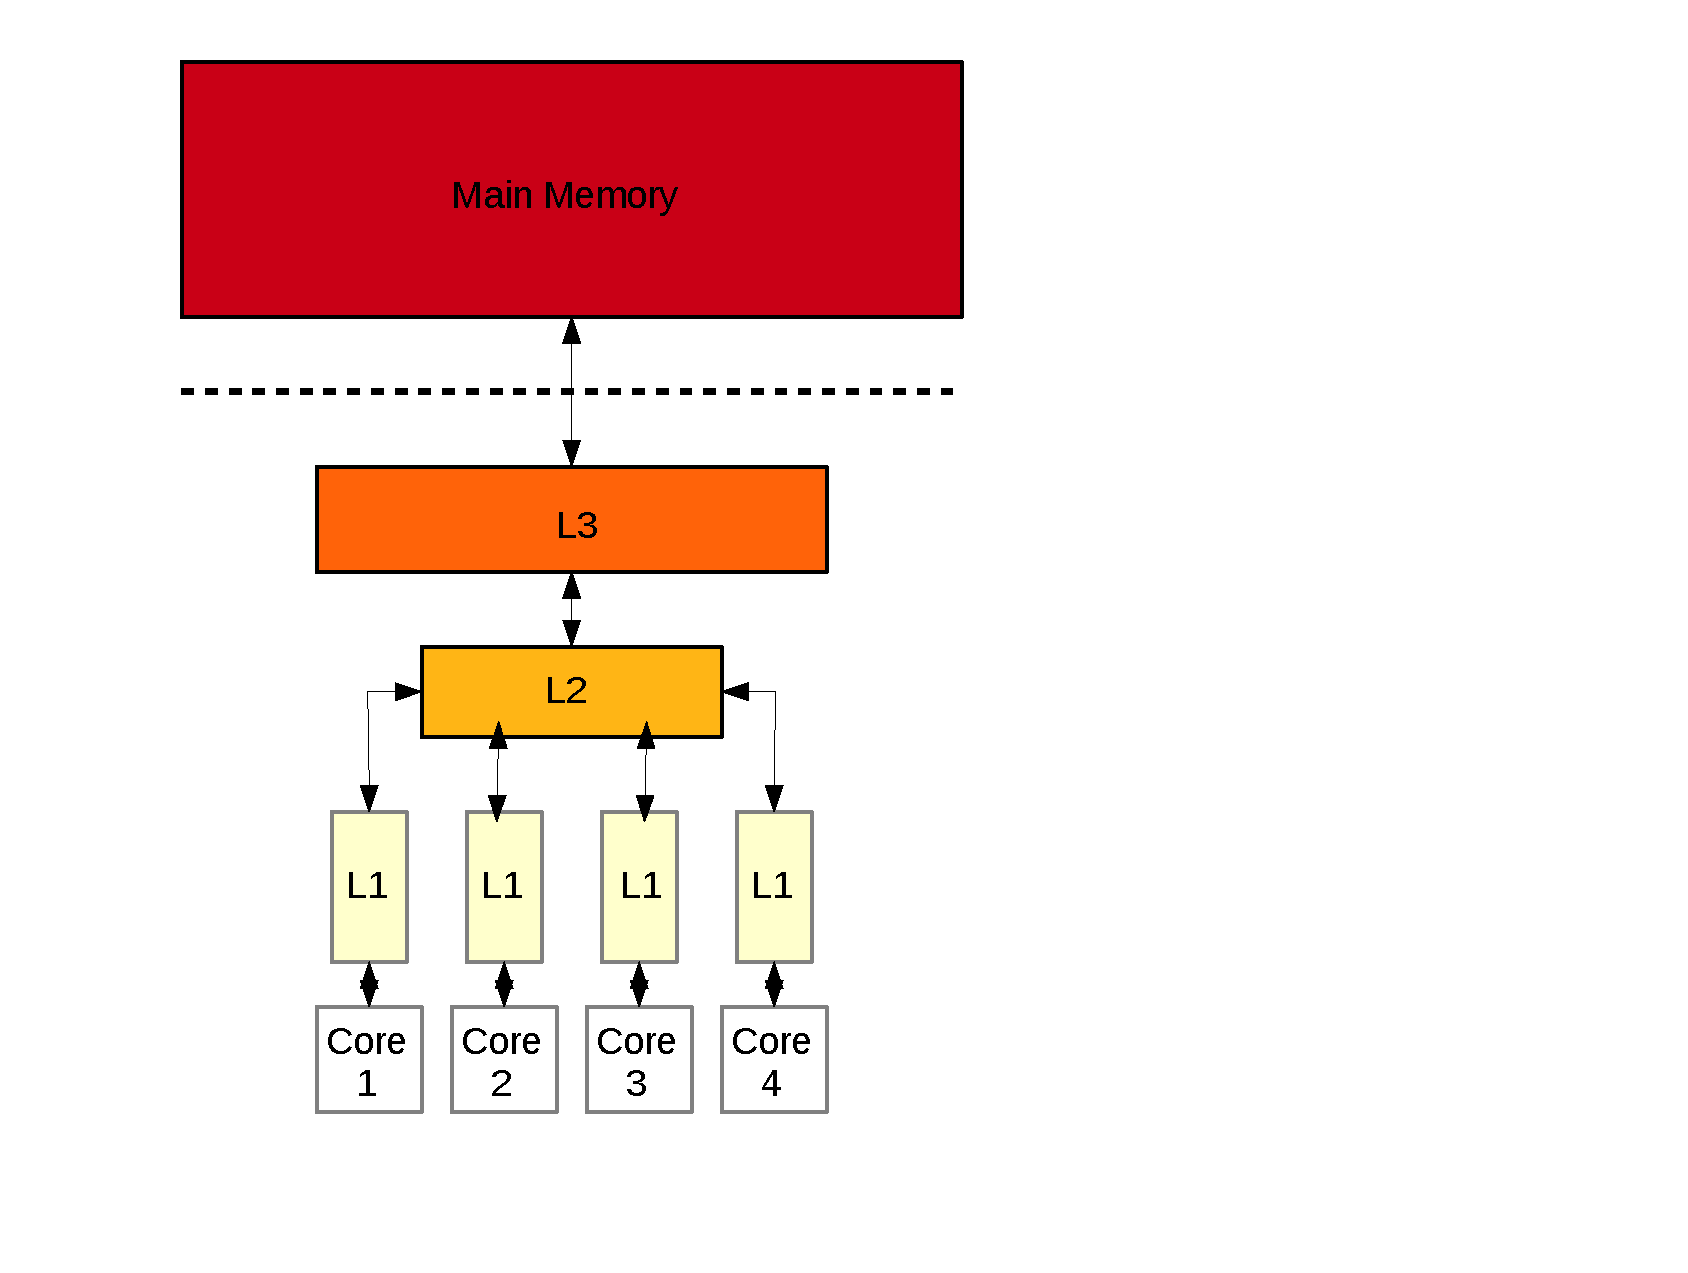
\includegraphics[width=1.0\textwidth]{cache}
	\caption{Typical memory hierarchy of modern computers.}
	\label{fig:cache}
\end{figure}

%%%%%%%%%%%%%%%%%%%%%%%%%%%%%%%%%%%%%%%%%%%%%%%%%%%%%%%%%%%%%%%%%%%%%%%%%%%%%%%%
% Step 12: Here's the main part of your research project. We can't tell
% you what to write here... that's your job.
% 
%%%%%%%%%%%%%%%%%%%%%%%%%%%%%%%%%%%%%%%%%%%%%%%%%%%%%%%%%%%%%%%%%%%%%%%%%%%%%%%%
\chapter{Planification}\label{chap:planification}

Image ~\ref{fig:plan} shows the planification of work for this project.

\begin{figure}[h!]
  \centering
    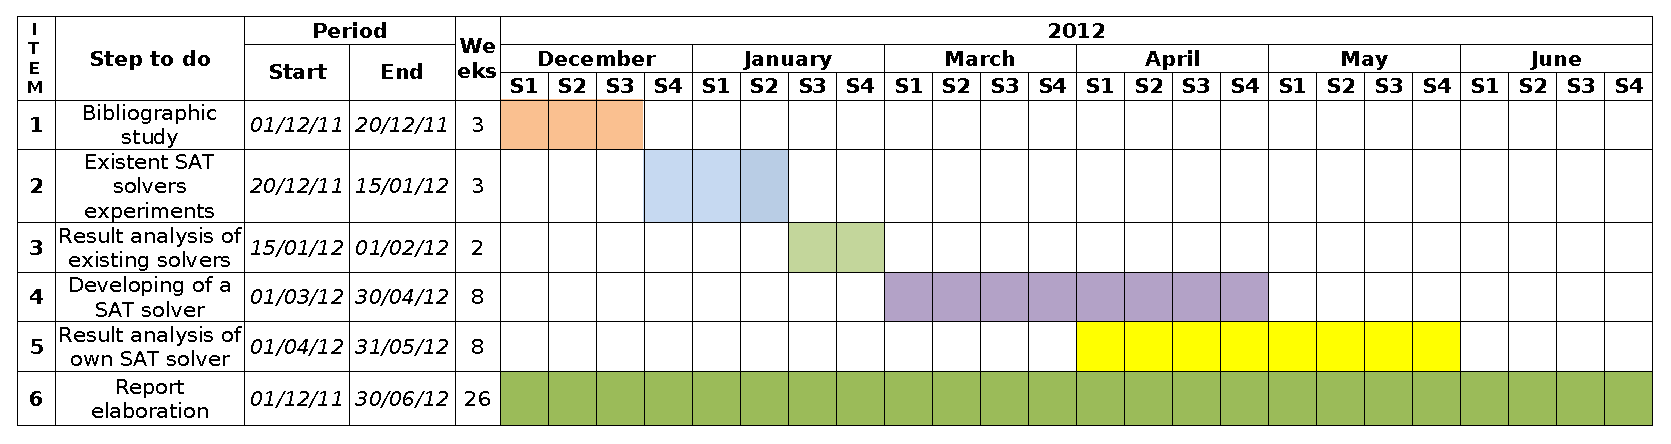
\includegraphics[angle=90, scale=0.6]{plan}
  \caption{Planification of work to be done in the project.}
  \label{fig:plan}
\end{figure}

%%%%%%%%%%%%%%%%%%%%%%%%%%%%%%%%%%%%%%%%%%%%%%%%%%%%%%%%%%%%%%%%%%%%%%%%%%%%%%%%
% Step 13: Add a conclusions chapter
%
% 
%%%%%%%%%%%%%%%%%%%%%%%%%%%%%%%%%%%%%%%%%%%%%%%%%%%%%%%%%%%%%%%%%%%%%%%%%%%%%%%%

%%%%%%%%%%%%%%%%%%%%%%%%%%%%%%%%%%%%%%%%%%%%%%%%%%%%%%%%%%%%%%%%%%%%%%%%%%%%%%%%
% Step 14: Work out the bibliography
%
% 
%%%%%%%%%%%%%%%%%%%%%%%%%%%%%%%%%%%%%%%%%%%%%%%%%%%%%%%%%%%%%%%%%%%%%%%%%%%%%%%%
% Tips: 
%
% For named.bst, if I add a~\cite*{} it will add all the references I
% have in the bibliography file (whether they are referenced in the
% document or not)
%%%%%%%%%%%%%%%%%%%%%%%%%%%%%%%%%%%%%%%%%%%%%%%%%%%%%%%%%%%%%%%%%%%%%%%%%%%%%%%%
\bibliographystyle{plain}
\bibliography{biblio}

\end{document}
